% !TeX root = ../SPL-Challenges.tex
% !TeX spellcheck = en_US
\section{Dynamic Ball Handling Challenge}

This challenge is a follow-up to the Dynamic Ball Handling Challenge of RoboCup 2022 and for this new edition a few small things were changed, but especially the scoring was adjusted. The purpose of this challenge is to enhance skills in ball passing and handling, and in robot's movement estimation.  

\subsection{Challenge Goal}

Score a goal as the attacking team after two or more passes without letting the defending players touch the ball. To allow for fast attacks, each player should pass the ball to the next target without them having to walk back or turn around.

\subsection{Challenge Setup}

This challenge is executed on a standard SPL field with GameController and consists of three individual runs with time in between (the exact time is subject to the given scheduling) in which changes/adjustments to the code are allowed. Three attacking robots, provided by the challenged team, and three defending robots, operating a provided common image (see \cref{sec:Challenge_image}) from another team, are competing. For each run a new defending image will be randomly selected (if more than one image exists), so that all teams have to compete against the same image.

The defending robots have to be flashed and calibrated with the selected image for each run. Teams have to practice setting up defending robots.
It is preferable that all teams in a run play against the same robots with the same defender image. However, this is only possible if one team per round agrees to provide these robots in addition. In this case, it should be ensured that the common defenders are not actively used for more than \qty{10}{\minute} at a time, otherwise a forced break of \qty{10}{\minute} (like a half-time) must be introduced. This will be decided by the referee of this challenge.
Otherwise each team will be teamed with another team for a run. Following from this, each run is divided into two phases executed after each other. For the first phase of a run the first mentioned team brings their three attacking robots and the other team provides the defending team. During the second phase teams switch their robots respectively. 

All participating teams have to have their robots ready \qty{10}{\minute} before each challenge run starts. Attacking robots are not allowed to be modified afterwards for this run (except a robot breaks, but even than the code should remain the same except for some necessary parameters).

The robots are placed by the referees facing the opponent's half and they should allow a bit of randomness into the position same for all teams in this run.
\begin{description}
	\item[Attacker:] \textit{1st:} goal area front line; \textit{2nd:} near to center line left of center circle, but at least \qty{10}{\cm} in its own half; \textit{3rd:} next to center line right of center circle, but at least \qty{10}{\cm} in its own half.
	\item[Defender:] \textit{1st:} goalkeeper on the ground line between the two goal posts; \textit{2nd:} front line penalty area; \textit{3rd:} within center circle, but at least \qty{10}{\cm} in its own half; 
	\item[Ball:] On penalty spot of the attacking team's side
\end{description}

\begin{figure}[hb!]
	\begin{center}
		\leavevmode
		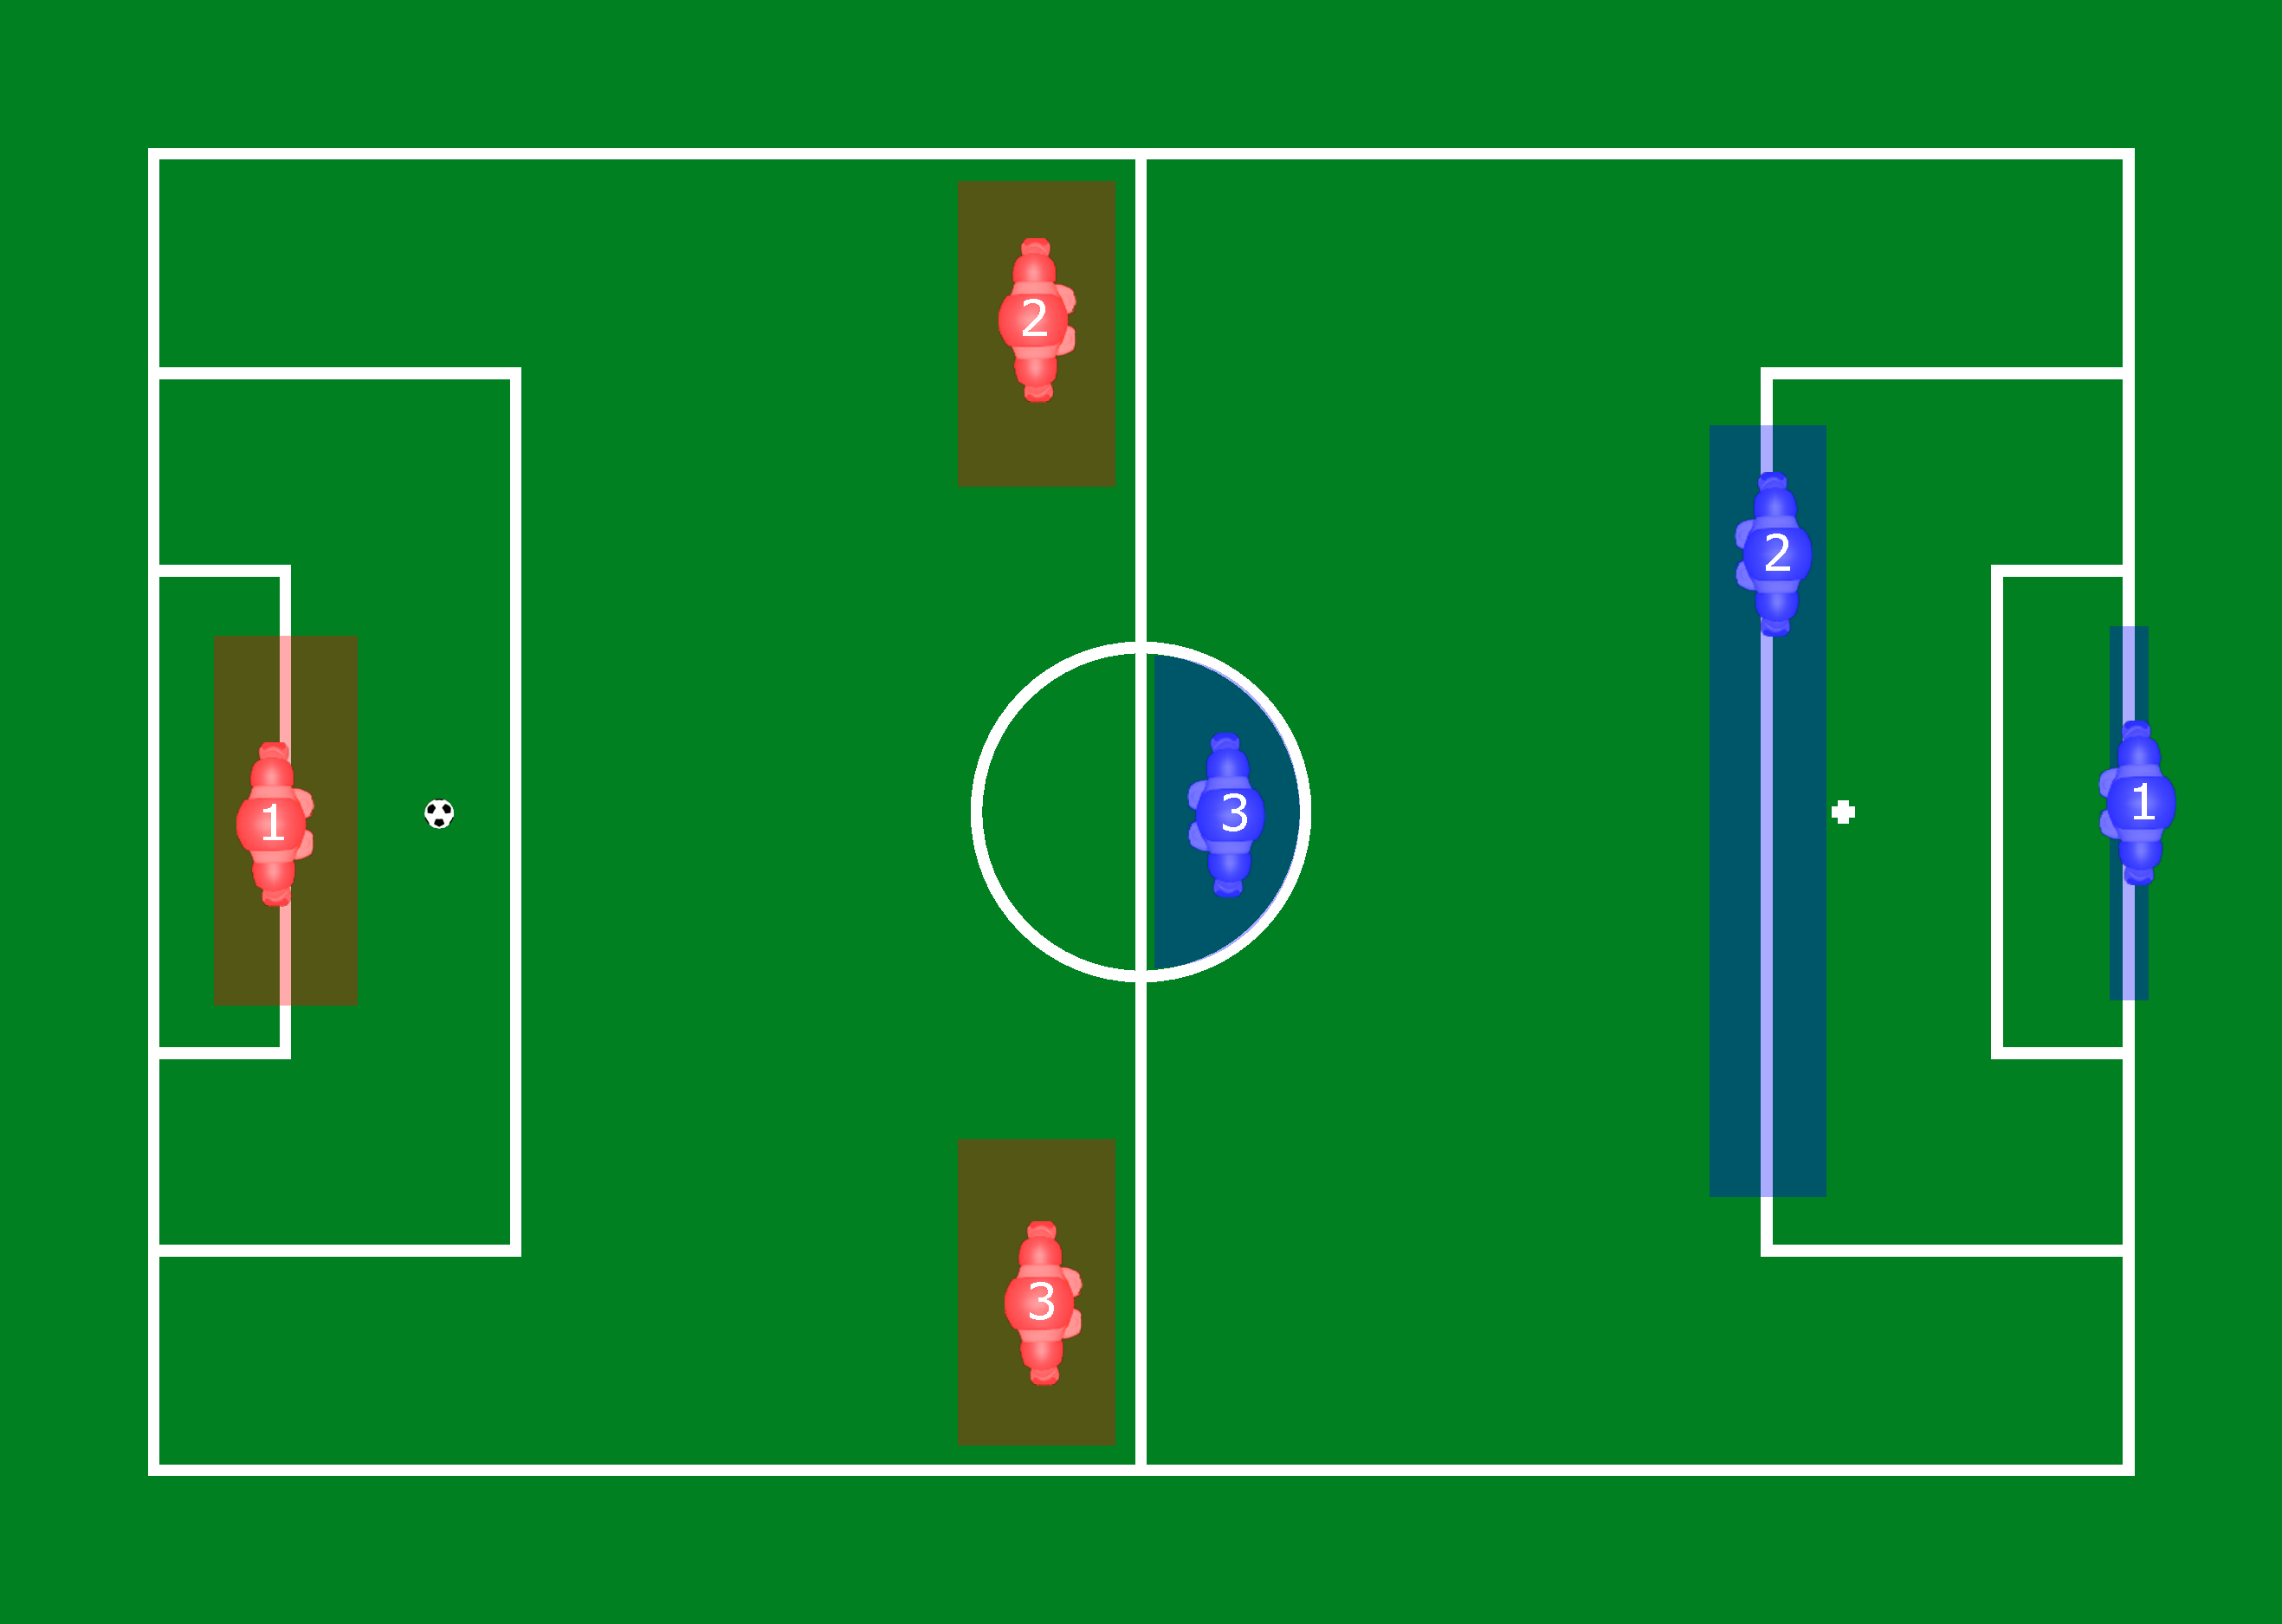
\includegraphics[width=1\columnwidth]{figs/dbhc_initial.pdf}
		\caption{Possible positions of the {\color{red}attacking (red)} and {\color{blue}defending (blue)} robots at the beginning of the challenge. All robots are facing their opponent's half and the possible randomized area is highlighted under the robots.}
		\label{fig:ball_handling_inital_positions}
	\end{center}
\end{figure}

\subsection{GameController}
All robots have to communicate with the GameController. There is a special mode in the GameController for this challenge. 

\subsection{Challenge Execution}

In \texttt{Initial} the robots get placed by the referees at their randomized starting positions, \cf~\cref{fig:ball_handling_inital_positions}. The GameController switches/skips from \texttt{Ready} directly into \texttt{Set}. The ball gets placed, and the head referee starts the run with one whistle blow, like at kick-off. If a robot does not listen to the whistle, it will receive the \texttt{Playing} signal from the GameController after the normal delay.

In \texttt{Playing} the teams have now \qty{240}{\second} time and the following happens: All robots are allowed to move and dribble. The 1st attacker passes the ball towards the 2nd or 3rd attacker while he is under attack by the 1st defender. After the 2nd or 3rd attacker received the ball, and the ball is in the defender's half, it gets attacked by the 2nd defender. Next, the 2nd or 3rd attacker passes towards the other robot, which can pass again or tries to score a goal.

Defending robots are limited to a maximum speed of \qty{200}{\mm \per \second}. Also the defenders are not allowed to listen/react to the whistle and only get the \qty{15}{\second} delayed \texttt{Playing} signal from the GameController! The 1st defender has to walk immediately into the attackers half and does not walk back in its own half, so it only defends in the attacker's half. The 2nd defender is only allowed to stay in its own half and the goalkeeper remains on the goal line and is not allowed to dive. The objective of the defending team is to intercept the passes, see~\cref{sec:Challenge_scoring}.

When the ball has been kicked by a robot who has a minimum distance to the receiving robot of \qty{2.0}{\metre} it is called a pass and then differentiated into the following categories:
\begin{enumerate}
	\item \textbf{substantial pass attempt}:
	\begin{enumerate}
		\item The ball stops in a circle with radius \qty{2.0}{\metre}, but greater \qty{1.0}{\metre}, around the receiver.
	\end{enumerate}
	\item \textbf{semi-valid pass}:
	\begin{enumerate}
		\item The ball stops in a circle with radius \qty{1.0}{\metre} around the receiver, but not within the arc defined in the next point.
	\end{enumerate}
	\item \textbf{valid pass}:
	\begin{enumerate}
		\item The ball stops in an \qty{180}{\degree} arc with radius~\qty{1.0}{\metre} around the receiver facing the next target, either next receiver or opponent's goal, so the receiving robot does not have to move backwards to pass or shoot a goal (\cf~\cref{fig:ball_handling_arc_positions}).
		\item The ball is without stoppage played in the direction of the next target, either next receiver or opponent's goal. Target direction is defined as a \qty{90}{\degree} cone towards the next target.
		\item The ball gets \textit{intentionally} deflected by the receiving robot in the direction of the next target either next receiver or opponent's goal. Target direction is defined as a \qty{90}{\degree} cone towards the next target.
	\end{enumerate}
\end{enumerate}

All rules from the normal game play (including penalties) still apply. Only the standard removal penalty time gets extended to \qty{240}{\second}. 
%If a defender pushes an attacking robot, the attacking team gets a time bonus of \qty{15}{\second}.

\begin{figure}[ht!]
	\begin{center}
		\leavevmode
		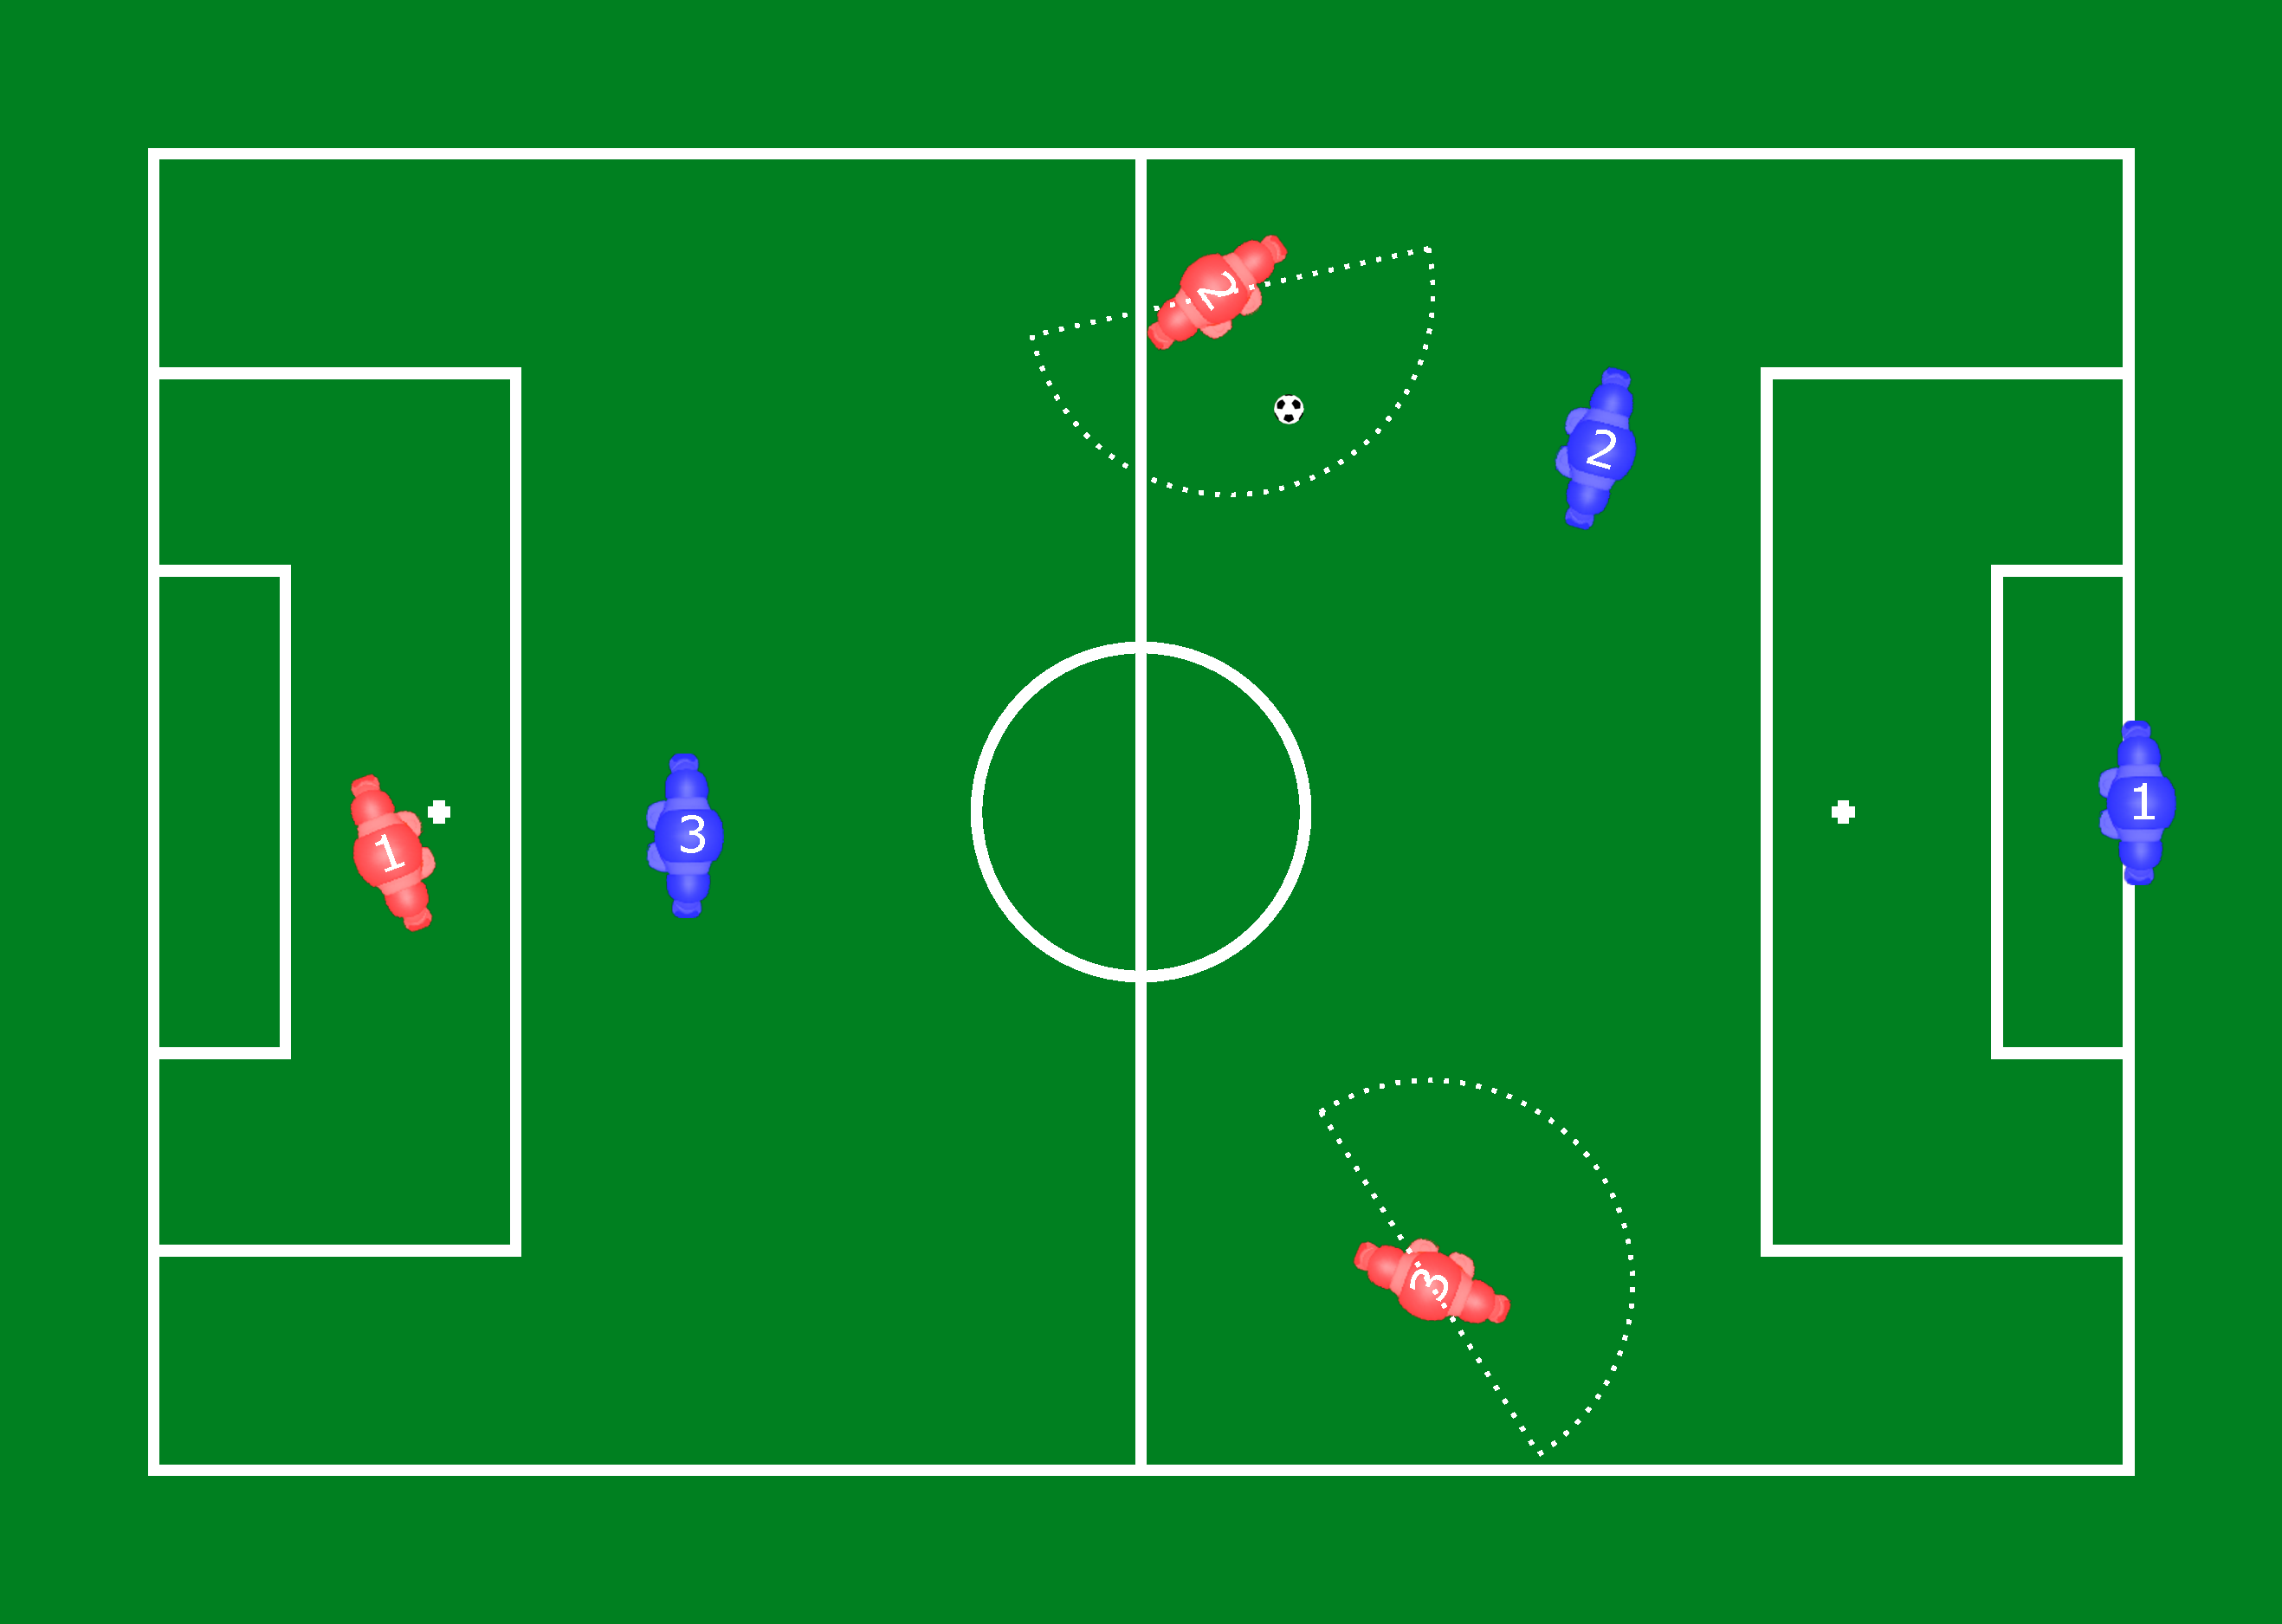
\includegraphics[width=1\columnwidth]{figs/dbhc_arcs.pdf}
		\caption{Possible challenge situation with {\color{red} attacking (red)} robots already oriented towards their targets. The arcs for a valid pass are indicated with dashed line style. Please note the possible difference between robot orientation and valid arcs.}
		\label{fig:ball_handling_arc_positions}
	\end{center}
\end{figure}

\subsection{Challenge Scoring}
\label{sec:Challenge_scoring}
In each run the GameController measures the execution time from initial whistle until the run is stopped by one of the following criteria:

\begin{itemize}
	\item A goal is scored after at least two passes, out of the following list, have been executed:
	\begin{itemize}
		\item valid pass,
		\item semi-valid pass,
		\item substantial pass attempt.
	\end{itemize}
	\item A defender (except the goalkeeper) touches the ball.
	\item Ball leaves the field outside the defending goal area.
	\item An attacker pushes.
	\item There is only one attacker left on the field.
	\item A run exceeds \qty{4}{\minute} execution time.
	\item Attacking team is not communicating with the GameController.
\end{itemize}

In the case that a goal gets scored before two passes (see list above) were executed, or the ball leaves the field within the defending goal area, the ball gets placed on the closest goal kick spot.

The score for the attacking team in a run will be calculated based on the following rules:

\begin{enumerate}
	\item For the first two passes, add 
	\begin{enumerate}
		\item \textbf{valid pass}: \qty{30}{} points.
		\item \textbf{semi-valid pass}: \qty{20}{} points.
		\item \textbf{substantial pass attempt}: \qty{10}{} points.
	\end{enumerate}
	\item For a third pass, add
	\begin{enumerate}
		\item \textbf{valid pass}: \qty{20}{} points.
		\item \textbf{semi-valid pass}: \qty{13}{} points.
		\item \textbf{substantial pass attempt}: \qty{6}{} points.
	\end{enumerate}
	\item For a fourth pass, add
	\begin{enumerate}
		\item \textbf{valid pass}: \qty{10}{} points.
		\item \textbf{semi-valid pass}: \qty{6}{} points.
		\item \textbf{substantial pass attempt}: \qty{3}{} points.
	\end{enumerate}
	\item For a goal after at least two passes, add \qty{50}{} points.
	\item The time measured counts and can lead to \qty{120}{} points if \qty{0}{\second} are needed and \qty{0}{} points if \qty{240}{\second} are needed. In between full points (rounded) will be awarded linearly. \\
	\textit{However these points are not awarded if the run was stopped by a stopping criteria different to scoring a goal, see above.}
	\item If an attacking robot has been pushed by a defender, subtract \qty{20}{\second} of the time measured.
\end{enumerate}

The final score is the sum of the two best runs out of the three runs.

\subsection{Defender image}
\label{sec:Challenge_image}
Common defender images can be provided by the community with a standardized setup procedure and with automatic calibration. Every team can propose such an image until 2023-05-14. The image will be tested until 2023-05-31 if they match the requirements and afterwards published. If not, the team gets feedback and has the opportunity to hand in a revised image. If teams want to test their attackers before this deadline the old images from 2022 and the old GameController can be used.

\begin{enumerate}
	\item One image applying to the standard button interface, using autonomous calibration and receives it player number through a text file on USB-stick.
	\item Existence of documentation on how to flash, how to operate a robot, how to handle issues.
	\item Does it apply to the rules?
	\item Does it operate robustly?
	\item Does it defend according to the rules?
\end{enumerate}
